70. $y=\cfrac{3x^2-6x}{|x-1|-1}=\begin{cases}\cfrac{3x(x-2)}{x-2}=3x,\ x\geqslant1,\ x\neq2,\\ \cfrac{3x(x-2)}{-x}=6-3x,\ x<1,\ x\neq0.\end{cases}$
$$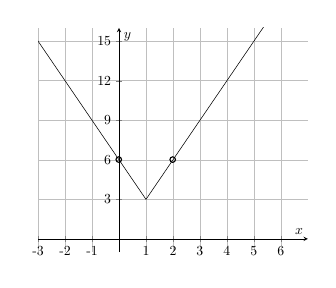
\begin{tikzpicture}[scale=0.5]
\begin{axis}[
    axis lines = middle,
    grid=major,
    legend pos={south west},
    xlabel = {$x$},
    %xlabel style={below right},
    ylabel = {$y$},
    ymin=-1,
    ymax=16,
    xmin=-3,
    xmax=7,
    xtick={-3,-2,-1,1,2,3,4,5,6},
    xticklabels={-3,-2,-1,1,2,3,4,5,6},
    ytick={3,6,9,12,15},
    yticklabels={3,6,9,12,15},
                  ]
	\addplot[domain=-3.5:1, samples=100, color=black] {3*(2-x)};
    \addplot[domain=1:5.5, samples=100, color=black] {(3*x)};
        %\addplot[domain=2.01:6, samples=100, color=black] {2/(2-x)};
   % \addplot[domain=-3:3, samples=100, color=black] {-x};
     %\addlegendentry{$\text{Рис. 1}$};
\end{axis}
\draw (2.05,2.35) circle (2pt);
\draw (3.42,2.35) circle (2pt);
\end{tikzpicture}$$
По графику найдём значение $y=3.$\\
